%%%%%%%%%%%%%%%%%%%%%%%%%%%%%%%%%%%%%%%%%%%%%%%%%%%%%%%%%%%%%%%%%%%%%%%%%%%%%
%	e-Yantra, IIT-Bombay

%	Document Author: Bhumika Varshney
%	Date: 6th july,2015

%%%%%%%%%%%%%%%%%%%%%%%%%%%%%%%%%%%%%%%%%%%%%%%%%%%%%%%%%%%%%%%%%%%%%%%%%%%%%

\documentclass[table,10pt,red]{beamer} 
% change the alerted colour to blue
\setbeamercolor{alerted text}{fg=blue}

\usetheme{berlin}
% theme split

\usepackage{beamerthemesplit}
\usepackage{xcolor}
\usepackage{booktabs,array}
\usepackage{listings}
\usepackage{hyperref}
\usepackage{verbatim,moreverb}

\usepackage{colortbl}
\usepackage{multirow}
\usepackage{tikz}
\usetikzlibrary{arrows}


% theme shadow
\usepackage{beamerthemeshadow}

% For including figures
\usepackage{graphicx}

% logo
\logo{
\includegraphics[height=1cm]{iitblogo.pdf}}


% sf family, bold font
\sffamily \bfseries
% Beginning of title page
\title
% content inside [] appears at bottom of all page. content inside {} appears on first page as title. double backslash means line change 
[
	Firebird LPC2148 Robotics Research Platform	% bottom
	\hspace{0.5cm}
	\insertframenumber/\inserttotalframenumber
]
{
	Motion Control Of Firebird-V Robot
}

\author
[
	www.e-yantra.org
]
{
	e-Yantra Team \\
  Embedded Real-Time Systems Lab\\
  Indian Institute of Technology-Bombay \\
}
\date
{
IIT Bombay \\ {\today}
}
 
 
\begin{document} 

% Slide-1: Title Page
\begin{frame}
	\titlepage
\end{frame} 

% Slide-2: Agenda for Discussion
\section*{Outline}
\begin{frame}
	\frametitle{Agenda for Discussion}
	\tableofcontents
\end{frame} 

\section{Basic Movements of Robot}
\subsection{Motion of Robot}
% Slide-3: Motion of Robot
\begin{frame}
	\frametitle{Various Motion} \pause
	\begin{columns}
% First Column	
\pause
	\column{0.5\textwidth}
	
		\begin{minipage}[r]{0.5\textwidth} \pause
		\begin{tikzpicture}
		
		%\draw[help lines] (0,0) grid(5,5);
		\onslide <2->	\draw[->][thick,red,line width = 0.1cm] (-0.5,0.2)--(-0.5,1);
		\onslide <1->	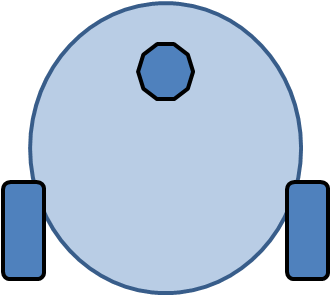
\includegraphics[width = 0.8\textwidth]{robot}
		\onslide <2->	\draw[->][thick,red,line width = 0.1cm] (0.5,0.2)--(0.5,1); 
		\end{tikzpicture}
		\vskip10pt \centering \textbf{Forward}\pause
		\end{minipage}
		\vfill 
		
		\begin{minipage}[c]{0.5\textwidth} 
		\vskip2cm
		\begin{tikzpicture} \pause
		%\draw[help lines] (0,0) grid(5,5);
		\onslide <5->\draw[<-][thick,red,line width = 0.1cm] (-0.5,0.2)--(-0.5,1);
		\onslide <4->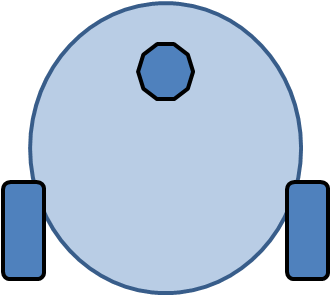
\includegraphics[width = 0.8\textwidth]{robot}
		\onslide <5->\draw[<-][thick,red,line width = 0.1cm] (0.5,0.2)--(0.5,1); 
		\end{tikzpicture}
		\vskip10pt \centering \textbf{Backward}\pause
		\end{minipage}
	\pause
	
% 2nd Column	
	\column{0.5\textwidth}
	\begin{minipage}[c]{0.5\textwidth} \pause
		\begin{tikzpicture}
		%\draw[help lines] (0,0) grid(5,5);
		\onslide <8->\draw[<-][thick,red,line width = 0.1cm] (-0.5,0.2)--(-0.5,1); 
		\onslide <7->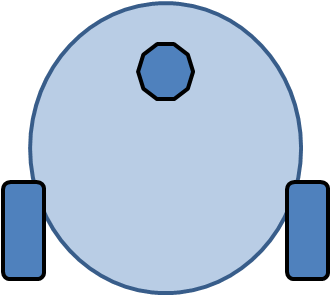
\includegraphics[width = 0.8\textwidth]{robot} 
		\onslide <8->\draw[->][thick,red,line width = 0.1cm] (0.5,0.2)--(0.5,1); 
		\end{tikzpicture}
		\vskip10pt \centering \textbf{Left}\pause
		\end{minipage}
		\vfill 
		
		\begin{minipage}[c]{0.5\textwidth} \pause
		\vskip2cm
		\begin{tikzpicture}
		%\draw[help lines] (0,0) grid(5,5);
		\onslide <11->\draw[->][thick,red,line width = 0.1cm] (-0.5,0.2)--(-0.5,1);
		\onslide <10->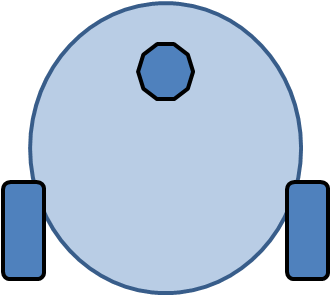
\includegraphics[width = 0.8\textwidth]{robot}
		\onslide <11->\draw[<-][thick,red,line width = 0.1cm] (0.5,0.2)--(0.5,1); 
		\end{tikzpicture} 
		\vskip10pt \centering \textbf{Right}\pause
		\end{minipage}
	\end{columns}
\end{frame}

% Slide-4: Motion of Robot
\begin{frame}
	\frametitle{Various Motion (Contd..)} \pause
	\begin{columns}
% First Column	
\pause
	\column{0.5\textwidth}
	
		\begin{minipage}[r]{0.5\textwidth} \pause
		\begin{tikzpicture}
		%\draw[help lines] (0,0) grid(5,5);
		\onslide <2->	\draw[->][thick,red,line width = 0.1cm] (-0.5,0.2)--(-0.5,1);
		\onslide <1->	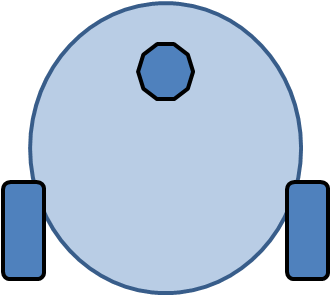
\includegraphics[width = 0.8\textwidth]{robot}
		%\onslide <2->	\draw[->][thick,red,line width = 0.1cm] (0.5,0.2)--(0.5,1); 
		\end{tikzpicture}
		\vskip10pt \centering \hskip15pt \textbf{Soft-Right} \pause
		\end{minipage}
		\vfill 
		
		\begin{minipage}[c]{0.5\textwidth} \pause
		\vskip2cm
		\begin{tikzpicture} 
		%\draw[help lines] (0,0) grid(5,5);
		%\onslide <5->\draw[<-][thick,red,line width = 0.1cm] (-0.5,0.2)--(-0.5,1);
		\hskip28pt
		\onslide <4->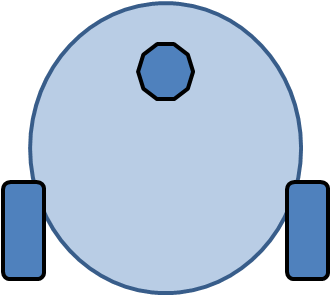
\includegraphics[width = 0.8\textwidth]{robot}
		\onslide <5->\draw[->][thick,red,line width = 0.1cm] (0.5,0.2)--(0.5,1); 
		\end{tikzpicture} 
		\vskip10pt \centering \hskip15pt \textbf{Soft-Left} \pause
		\end{minipage}
	\pause
	
% 2nd Column	
	\column{0.5\textwidth}
	\begin{minipage}[c]{0.5\textwidth} \pause
		\begin{tikzpicture}
		%\draw[help lines] (0,0) grid(5,5);
		\onslide <8->\draw[<-][thick,red,line width = 0.1cm] (-0.5,0.2)--(-0.5,1); 
		\onslide <7->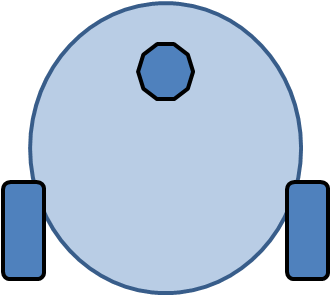
\includegraphics[width = 0.8\textwidth]{robot} 
		%\onslide <8->\draw[->][thick,red,line width = 0.1cm] (0.5,0.2)--(0.5,1); 
		\end{tikzpicture}
		\vskip10pt \centering \hskip10pt \textbf{Backward Left}\pause
		\end{minipage}
		\vfill 
		
		\begin{minipage}[c]{0.5\textwidth} \pause
		\vskip2cm
		\begin{tikzpicture}
		%\draw[help lines] (0,0) grid(5,5);
		%\onslide <11->\draw[->][thick,red,line width = 0.1cm] (-0.5,0.2)--(-0.5,1);
		\hskip28pt
		\onslide <10->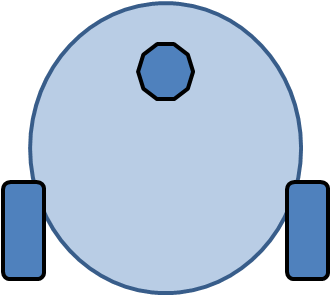
\includegraphics[width = 0.8\textwidth]{robot}
		\onslide <11->\draw[<-][thick,red,line width = 0.1cm] (0.5,0.2)--(0.5,1); 
		\end{tikzpicture}
		\vskip10pt \centering  \hskip3pt \textbf{Backward Right}\pause
		\end{minipage}
	\end{columns}
\end{frame}

% Slide-5: Direction Control of DC Motor
\begin{frame}{Direction Control of DC Motor}
	\begin{minipage}[c]{0.4\textwidth}\pause
		Anti-Clockwise Motion	\\[10pt]
			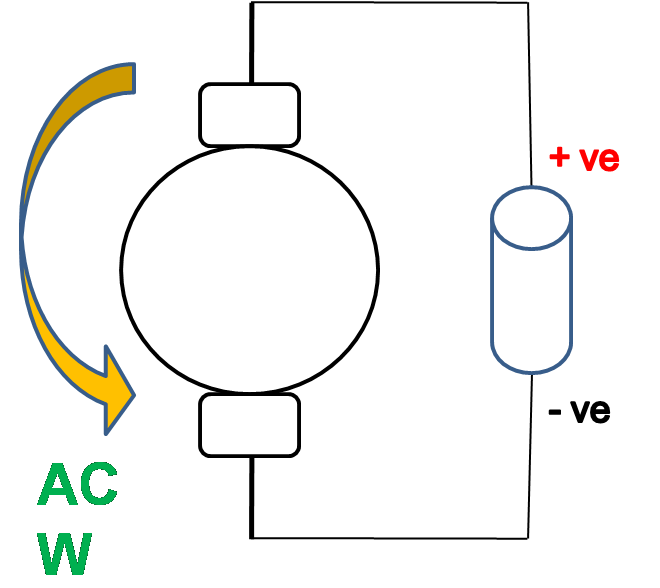
\includegraphics[width=\linewidth]{Motor_ACW}
		\end{minipage}
	\hfill \pause
	\begin{minipage}[c]{0.4\textwidth}\pause
			Clockwise Motion	\\[10pt]
			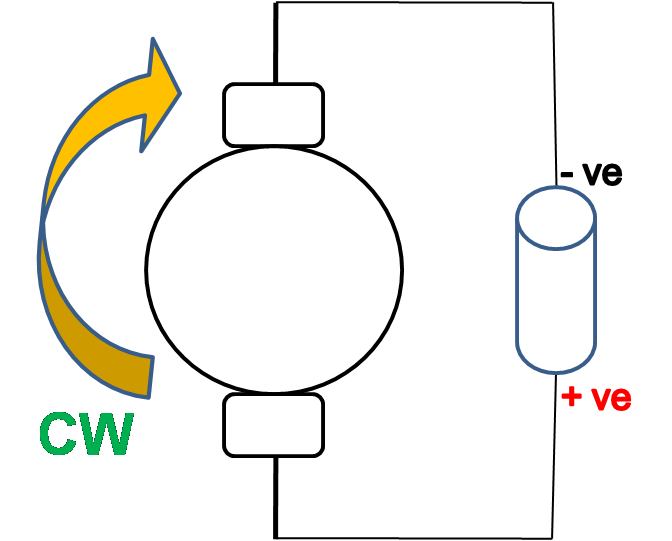
\includegraphics[width=\linewidth]{Motor_CW}
		\end{minipage}
	\hfill
\end{frame}


\subsection{Understanding L293D IC}
% Slide-6: L293D IC
	\begin{frame}
		\frametitle{L293D IC}	\pause
			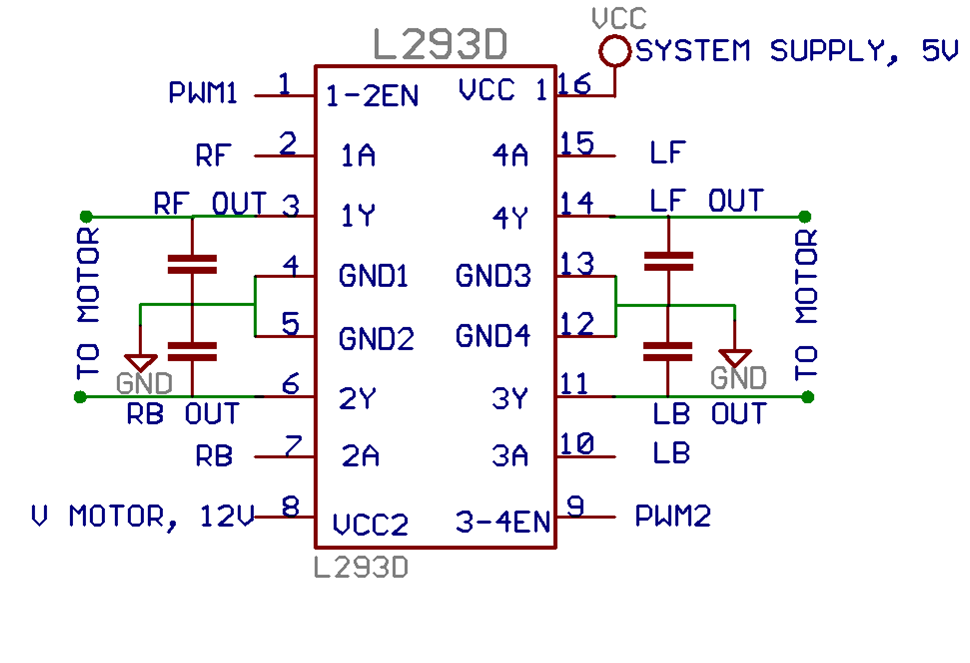
\includegraphics[width=\linewidth]{L293D}
	\end{frame}
	
\section{Motor Interfacing on Firebird}
	
\subsection{Pin connections}
% Slide-7: Motor Pin Connection
	\begin{frame}
		\frametitle{Motor Pin Connection}	\pause
			\begin{enumerate}
				\item <+-|alert@+> Three out of four pins for Direction control is connected at PORT0 and one pin is connected at PORT1\pause \\[10pt]
				\begin{enumerate}[a.]
					\item <1-> P0.22 - Left Motor Control\\[10pt]
					\item <1-> P1.21 - Left Motor Control\\[10pt]
					\item <2-> P0.10 - Right Motor Control\\[10pt]
					\item <2-> P0.11 - Right Motor Control\\[10pt]
				\end{enumerate} \pause
			\item <+-|alert@+> Two Pins for Enabling Motor Driver IC is connected at PORT0 \pause\\[10pt]
			\begin{enumerate}[a.]
					\item <1-> P0.7 (PWM2)- Left Channel Enable\\[10pt]
					\item <2-> P0.21 (PWM5)- Right Channel Enable\\[10pt]
			\end{enumerate}
			\end{enumerate}	
	\end{frame}

\subsection{Logic Table}
% Slide-8: Logic Table
	\begin{frame}
	\frametitle{Logic Table} \pause
	%\rowcolors{1}{gray}{white}
	\centering
		\begin{tabular}{!{\vrule width 2pt}c|c|c|c|c!{\vrule width 2pt}}
				\noalign{\hrule height 2pt} 
				\multirow{2}{*}{Direction} & P0.22 & P1.21 & P0.10 & P0.11\\[2pt] 
																	 & LB & LF & RF & RB 	\\ 
				\noalign{\hrule height 1pt} \pause 
				Forward\pause&0&\color{red}1&\color{red}1&0 \\
				\hline \pause
				Backward\pause&\color{red}1&0&0&\color{red}1\\
				\hline \pause
				Left\pause&\color{red}1&0&\color{red}1&0\\
				\hline \pause
				Right\pause&0&\color{red}1&0&\color{red}1\\
				\hline \pause
				Soft Left\pause&0&0&\color{red}1&0\\
				\hline \pause
				Soft Right\pause&0&\color{red}1&0&0 \\
				\hline \pause
				Stop\pause&0&0&0&0\\
				\hline
				\noalign{\hrule height 2pt}													 
		\end{tabular}
	\end{frame}

\subsection{Writing C-Code}
% Slide-9: Syntax for C-Program
\begin{frame}[shrink = 2,fragile] 
	\frametitle{Syntax for C-Program}\pause
	
		\begin{block}<1->{\#include}\pause
		\begin{semiverbatim}
				#include <lpc214x.h>
 		\end{semiverbatim}
		\end{block} \pause
		
	\begin{block}<2->{Pin Configuration}\pause
		\begin{semiverbatim}
				void Init_motion_pin (void)
				\{
 			\ \ \		PINSEL0 = 0X00002000;	\color{red}// Set direction pins as GPIOs  \color{black}		
 			\ \ \		PINSEL1 = 0x00000400;
 			\ \ \ PINSEL2 = 0x00000000;
 			\ \ \		IO0DIR  = 0x00600C80;  \color{red}// Output Port0 \color{black}		
 			\ \ \		IO1DIR  = 0x00200000;  \color{red}// Output Port1 \color{black}		
 			\ \ \		IO0SET  = 0x00200080; 	\color{red}// Set PWM Pins \color{black}
 			\ \ \		IO0CLR  = 0x00400C00;	\color{red}// Initially stop \color{black}
 			\ \ \		IO1CLR  = 0x00200000;
 				\}
 		\end{semiverbatim}
		\end{block}	
\end{frame}

% Slide-10: Syntax for C-Program (Contd..)
\begin{frame}[shrink = 4,fragile]
	\frametitle{Syntax for C-Program (Contd..)} \pause
	
		\begin{block}<1->{Main-Program}	\pause
		\begin{semiverbatim}
				int main (void) 
				\{
			\ \		 Init_motion_pin ();
			\ \		 while(1)
			\ \	 	\{
			\ \ \ \ \ \				forward();
			\ \ \ \ \ \				delay_ms();
			\ \ \ \ \ \				stop();
			\ \ \ \ \ \				delay_ms();
			\ \	 	\}	
				\}	
			\end{semiverbatim}
		\end{block} \pause
	
	\begin{block}<2->{Functions}\pause
		\begin{semiverbatim}
				void forward (void)
				\{
 		\ \ \		IO0SET= (1<<10);
		\ \ \	 	IO1SET=(1<<21);
		\ \ \	 	IO0CLR=(1<<22)|(1<<11);		
				\}
				
				\hrule \hrule	\pause
				void stop (void)
				\{
 		\ \ \		IO0CLR=(1<<10)|(1<<11)|(1<<22);
		\ \ \	 	IO1CLR=(1<<21);		
				\}
 		\end{semiverbatim}
	\end{block}
\end{frame}

% Slide-11: Syntax for C-Program (Contd..)
\begin{frame}
	\frametitle{Syntax for C-Program (Contd..)} \pause
	Define All related motion functions and include in main function \pause\\[10pt]
	\begin{enumerate}
		\item <+-|alert@+> Backward();\\[10pt]
		\item <+-|alert@+> Right();\\[10pt]
		\item <+-|alert@+> Left();\\[10pt]
		\item <+-|alert@+> Soft Right();\\[10pt]
		\item <+-|alert@+> Soft Left();\\[10pt]	
	\end{enumerate}
	
\end{frame}

\begin{frame}
% Slide-12: Last Slide
\hskip4cm
\textbf{\LARGE Thank You!} \\[20pt]
\hskip3cm
\scriptsize Post your queries on: 
\hyperref[www.e-yantra.org]{\color{blue} http://qa.e-yantra.org/ \color{black}} 
\end{frame}

\end{document} 